\documentclass{ctexart}
\usepackage{graphicx}
\usepackage{xcolor}
\usepackage{amsmath}
\usepackage[colorlinks, linkcolor=red]{hyperref}
\begin{document}
	
	\section{概率论}
	
	\subsection{全概率公式以及贝叶斯公式}
	
	\textbf{条件概率}
	
	条件概率的定义是,设有两个事件A,B,而P(B) \(\neq\) 0,则在给定B发生的条件下A的条件概率记为P(A|B),定义为:
	
	\[P(A|B)=P(AB)/P(B), P(B) \neq 0\]
	
	对于公式的理解,条件概率是在B发生的条件下,也就是B发生的时候,A也发生,简言之就是在B发生的条件下A和B同时发生的概率。可以根据下图来帮助理解
	
	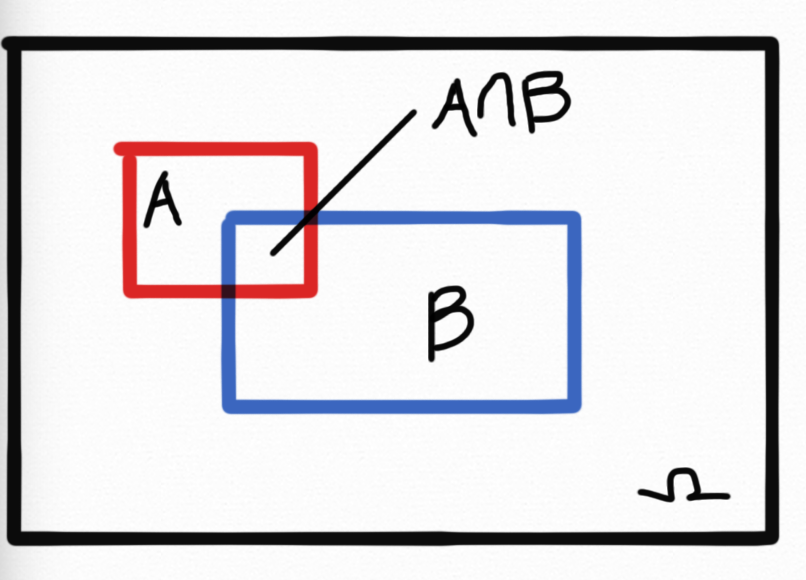
\includegraphics[width=0.8\linewidth]{pic/AB}
	
	\mbox{}
	
	\textbf{全概率公式}
	
	设\(B_1,B_2...\)为有限或无限个事件,它们两两互斥且在每次实验中至少发生一个,即:
	
	\[B_iB_j=\emptyset, i \neq j\]
	
	\[B_1+B_2+···· = \omega\]
	
	把具有这些性质的一组事件成为一个完备事件组。任一事件B以及其对立事件组成一个完备事件组。
	
	现考虑任一事件A。因\(\omega\)是必然事件,有\(A=A\omega=AB_1+AB_2+····\),因\(B_1,B_2,...\)两两互斥,显然\(AB_1,AB_2,...\)也两两互斥。
	
	由加法定理有
	
	\[P(A)=P(AB_1)+P(AB_2)+····\]
	
	再由条件概率的定义有:
	
	\[P(A)=P(B_1)P(A|B_1)+P(B_2)P(A|B_2)+···\]
	
	上式成为全概率公式。“全部”概率P(A)被分解成了许多部分之和,在较复杂的情况下直接算P(A)不容易,但A总是伴随着某个\(B_i\)伴出。
	
	另一角度理解,把\(B_i\)看作是导致事件A发生的一种可能途径,对不同的途径,A发生的概率即条件概率P(A|B)各个不同,而采取哪个途径却是随机的。
	
	\mbox{}
	
	\textbf{贝叶斯公式}
	
	根据条件概率的定义以及在全概率公式的假定下
	
	\[P(B_i|A)=P(AB_i)/P(A)=P(B_i)P(A|B_i)/\sum_{j}P(B_j)P(A|B_j)\]
	
	如果把事件A看成是“结果”,把诸事件\(B_1,B_2,...\)看成是导致这结果的可能的“原因”,则可以把全概率公式看作成为“由原因推导结果”;而贝叶斯公式看作是“由结果推导原因”:现在有一个结果A已经发生,在众多可能的原因中,是哪一个导致了这结果?
	
	\subsection{随即变量及概率分布}
	
	\textbf{一维随机变量}
	
	随机变量:顾名思义,就是其值随机会而定。可以说随机变量就是实验结果的函数。在实验前,我们不能预知它将取何值,这要凭机会,一旦试验后,取值就确定了。
	
	随机变量按其可能取值的全体的性质,分为两大类:
	
	一类叫离散型随机变量。{\color{red}其特征是只能取有限个值,或随在理论上能取无限个值,但这些值可以毫无遗漏地一个接一个排列出来。}
	
	另一类叫连续型随即变量,取值不仅是无穷多,{\color{red}还不能无遗漏地逐一排列,而是充满一个区间}。
	
	\mbox{}
	
	\textbf{离散型随机变量分布}
	
	\textbf{定义:}设X为离散型随机变量,其全部可能值为\(\{a_1,a_2,...\}\)则
	
	\[p_i=P(X=a_i), i =1,2,...\]
	
	称为X的概率函数,也成为概率分布
	
	\textbf{定义:}设X为一随机变量,则函数
	
	\[P(X \leq x)=F(x), -\infty < x < \infty\]
	
	称为X的分布函数。它对任何随即变量都有定义。
	
	若知道离散型的概率函数,则
	
	\[F(x)=P(X \leq x)=\sum_{\{i:a_i \leq x\}}p_i\]
	
	\textbf{连续型随机变量分布}
	
	\textbf{定义:}设连续性随机变量X有概率分布函数F(x),则F(x)的倒数\(f(x)=F^{'} (x)\),称为X的概率密度函数
	
	密度函数解释:取一个点x,则按分布函数的定义,事件\(\{x < X < \leq x+h\}\)的概率(h > 0为常数),应为F(x+h)-F(x),所以比值[F(x+h)-F(x)]/h可以解释为在x点附近h这么长的区间(x, x+h)内,单位长所占有的概率。令\(x \to 0\),则这个比的极限,即\(F^{'}=f(x)\),也就是在x点处单位长的概率,或者说它反映了概率在x点处的密集程度。
	
	\subsection{多维随机变量}
	
	\textbf{定义:}以\(\{a_{i1},a_{i2},...\}\)记\(X_i\)的全部可能值,i=1,2...则事件\(\{X_1=a_{1_{j_1}}, X_2=a_{2_{j_2}},...,X_n=a_{n_{j_n}}\}\)的概率
	
	\[p(j_1,j_2,...,j_n)=P(X_1=a_{1_{j_1}}, X_2=a_{2_{j_2}},...,X_n=a_{n_{j_n}})\]
	
	\[j_1=1,2,..., j_2=1,2,...., j_n=1,2,....\]
	
	称为随即向量\(X_1,...,X_n\)的概率函数或概率分布
	
	\textbf{定义:}若\(f(x_1,x_2,...,x_n)\)是定义在\(R^n\)上的非负函数,使对\(R^n\)中的任何集合A,有
	
	\[P(X \in A) = \int_A···\int f(x_1,...,x_n)dx_1···dx_2\]
	
	则称f是X的密度函数
	
	\mbox{}
	
	\textbf{边缘分布}
	
	设\(X=(X_1,...,X_n)\)是一n维随机变量,X有一定的分布F,这是一个n维分布。因为X的每个分量\(X_i\)都是因为随机变量,故它们有各自的分布\(F_i,i=1,2,...,n\),这些都是一维分布,成为随即向量X或其分布F的边缘分布
	
	虽然一个随即向量\(X=(X_1,...,X_n)\)的分布F足以决定其任一分量\(X_i\)的边缘分布\(F_i\),但反过来不对,即使知道了所有\(X_i\)的边缘分布,也不足以决定X的分布F。边缘分布只考虑了单个变量的情况,而未涉及它们之间的关系,而这个信息是包含在\((X_1,...,X_n)\)的分布之内的。边缘分布就是通常的分布,无特殊含义。
	
	\subsection{条件概率分布}
	
	一个随机变量或向量X的条件概率分布,就是在某种给定的条件下,X的概率分布。一般采取如下的形式:设有两个随机变量或向量X,Y,在给定Y取某个或某些值的条件下,去求X的条件分布。
	
	\mbox{}
	
	\textbf{离散型随机变量的条件概率分布}
	
	设\((X_1,X_2)\)为一个二维离散随机向量,\(X_1\)的全部可能取值为\(a_1,a_2,...\);\(X_2\)的全部可能取值为\(b_1,b_2,...\),而\((X_1,X_2)\)的联合概率分布为
	
	\[p_{ij}=P(X_1=a_i,X_2=b_j), i,j=1,2,...\]
	
	考虑\(X_1\)在给定\(X_2=b_j\)的条件下的条件分布,依条件概率的定义,有
	
	\[P(X_1=a_i|X_2=b_j)=P(X_1=a_i, X_2=b_j)/P(X_2=b_j)=p_{ij}/P(X_2=b_j)\]
	
	而根据边缘分布\(P(X_2=b_j)=\sum_{k}p_{kj}\),于是
	
	\[P(X_1=a_i|X_2=b_j)=p_{ij}/\sum_{k}p_{kj}, i=1,2,...\]
	
	\mbox{}
	
	\textbf{连续型随机变量的条件概率分布}
	
	设二维随机向量\(X=(X_1,X_2)\)有概率密度函数\(f(x_1,x_2)\),先考虑在限定\(a \leq x_2 \leq b\)的条件下,\(X_1\)的条件分布,有
	
	\[P(X_1 \leq x_1 | a \leq X_2 \leq b) = \frac{P(X_1 \leq x_1 , a \leq X_2 \leq b)}{P(a \leq X_2 \leq b)}\]
	
	\[P(X_1 \leq x_1 , a \leq X_2 \leq b)=\int_{\infty}^{x_1} dt_1\int_{a}^{b}f(t_1,t_2)dt_2\]
	
	\(X_2\)的边缘分布的密度函数\(f_2(x_2)=\int_{-\infty}^{\infty}f(x_1, x_2)dx_1\)
	
	\[P(a \leq X_2 \leq b) = \int_{a}^{b}f_2(t_2)dt_2\]
	
	由此可得
	
	\[P(X_1 \leq x_1 | a \leq X_2 \leq b)=\frac{\int_{\infty}^{x_1} dt_1\int_{a}^{b}f(t_1,t_2)dt_2}{\int_{a}^{b}f_2(t_2)dt_2}\]
	
	这是\(X_1\)的条件分布函数,对\(x_1\)求导,得到条件密度函数
	
	\[f_1(x_1| a \leq X_2 \leq b)=\int_{a}^{b}f(x_1, t_2)dt_2/\int_{a}^{b}f_2(t_2)dt_2\]
	
	若在给定a=b的情况下,即在\(X_2\)给定等于一个值之下,\(X_1\)的条件密度函数。
	
	\begin{align*}
	f_1(x_1|x_2) &= f_1(x_1|X_2=x_2) \\
					 & = \lim\limits_{h \rightarrow 0}f_1(x_1|x_2 \leq X_2 \leq x_2+h) \\
					 &= \lim\limits_{h \to 0}\frac{1}{h}\int_{x_2}^{x_2+h}f(x_1, t_2)dt_2/\lim\limits_{h \to 0}\frac{1}{h}\int_{x_2}^{x_2+h}f_2(t_2)dt_2 \\
				 	& = f(x_1, x_2)/f_2(x_2)
	\end{align*}
	
	式子改写成
	
	\[f(x_1, x_2)=f_2(x_1)f_1(x_1|x_2)\]
	
	就是说两个随机变量的联合概率密度,等于其中之一的概率密度乘以在给定这一个之下另一个的概率密度。
	
	式子可以推广到多个变量的场合:设有n维随机向量\(X_1,..,X_n\),其概率密度函数\(f(x_1,...,x_n)\)则
	
	\[f(x_1,...,x_n)=g(x_1,...,x_k)h(x_{k+1},...,x_n|x_1,...,x_k)\]
	
	其中g是\(X_1,...,X_k\)的概率密度,而h则是在给定\(X_1=x_1,...,X_k=x_k\)的条件下,\(X_{k+1},...,X_n\)的条件概率密度。
	
	\mbox{}
	
	\textbf{随机变量的独立性}
	
	\textbf{定义:}设n维随机向量\(\{X_1,...,X_n\}\)的联合密度函数为\(f(x_1,...,x_n)\),而\(X_i\)的边缘密度函数为\(f_i(x_i),i=1,2,...,n\)如果:
	
	\[f(x_1,...,x_n)=f_1(x_1)···f_n(x_n)\]
	
	就称随机变量\(\{X_1,...,X_n\}\)相互独立
	
	\mbox{}
	
	\textbf{定义:}设\(\{X_1,...,X_n\}\)都是离散型随机变量,若对任何常数\(a_1,...,a_n\)都有:
	
	\[P(X_1=a_1,...,X_n=a_n)=P(X_1=a_1)···P(X_n=a_n)\]
	
	就称随机变量\(\{X_1,...,X_n\}\)相互独立
	
	\subsection{随机变量的函数的概率分布}
	
	已知某个或某些随机变量\(X_1,...,X_n\)的分布,另有一些随机变量\(Y_1,...,Y_m\),它们都是\(X_1,...,X_n\)的函数:
	
	\[Y_i=g_i(X_i,...,X_n),i=1,...,m\]
	
	比如在数理统计中,\(X_1,...,X_n\)是原始的观察或试验数据,\(Y_1,...,Y_m\)则是为某种目的将这些数据加工而得到的量,成为统计量。比如\(X_1,...,X_n\)的算术平均值\(\overline{X}=(X_1,...,X_n)/n\). \(\overline{X}\)就是\(X_1,...,X_n\)的函数。
	
	两个重要的特殊函数:
	
	\(\Gamma\)函数\(\Gamma(x)\):通过积分
	
	\[\Gamma(x)=\int_{0}^{\infty}\exp^{-t}t^{x-1}dt, x > 0\]
	
	\[\Gamma(1)=1, \Gamma(1/2)=\sqrt{2}, \Gamma(x+1)=x\Gamma(x)\]
	
	\(\beta\)函数\(\beta(x,y)\):通过积分
	
	\[\beta(x,y)=\int_{0}^{1}t^{x-1}(1-t)^{y-1}, x > 0, y > 0\]
	
	\[\beta(x,y)=\Gamma(x)\Gamma(y)/\Gamma(x+y)\]
	
	
	
	\section{数理统计}
	
	\subsection{基本概念}
	当我们用试验或观察的方法研究一个问题时,首先要通过适当的观察或试验以取得必要的数据,然后对数据进行分析,以对所提出的问题作出尽可能正确的结论。
	
	之所以说尽可能正确,是因为数据一般带有随机性误差,不只是通常意义下得因测量不准造成的误差。由于数据带有随机误差,所以作出的结论,也有可能出错。
	
	统计的两大问题:参数估计和假设检验
	
	参数估计:比如模型为指数函数,估计参数\(\lambda\)为多少,从而求得平均值\(1/\lambda\),\(\lambda\)一般是未知的。所以可以从选取的样本计算样本的平均值来估计\(1/\lambda\)
	
	假设检验:假设不符合但被接受,假设符合但可能被拒绝
	
	总体:是指与所研究的问题有关的对象的全体构成的集合
	
	总体的概率分布:是指数分布还是正态分布等等,总体就是一个概率分布,只要服从同一概率分布,就可以视为同类总体。
	
	样本:是按一定的规定从总体中抽出的一部分个体。总体中的每一个个体有同等的被抽出的机会。
	
	统计量:完全由样本所决定的量。统计量只依赖于样本,而不能依赖于其它位置的量。{\color{red}特别是,它不依赖与总体分布中所包含的未知参数}。例如,设\(X_1+...+X_n\)是从正态总体\(N(\mu, \sigma^2)\)中取出的样本,则\(\overline{X} = (X_1+...+X_n)/n\)是统计量,因为它完全由样本决定,但\(\overline{X}-\mu\)不是统计量,因为\(\mu\)未知,\(\overline{X}-\mu\)不是完全由样本所决定。
	
	统计量可以看作是对样本的一种加工,它把样本中所含的(某一方面)的信息集中起来。例如\(\overline{X}\)可以用于估计未知的\(\mu\)。可以这样看:原始数据\(X_1,...,X_N\)中的每一个,都包含有\(\mu\)的若干信息,但这些事杂乱无章的,一经集中到\(\overline{X}\)就有了明确的概念。
	
	统计量有:样本均值\(\overline{X}=(X_1+...+X_n)/n\)
	
	样本方差\(S^2=\sum_{i=1}^{n}(X-\overline{X})^2/(n-1)\)
	
	样本矩,分为样本原点矩和样本中心矩。
	
	\[a_k=(X_1^k+....+X_n^k)/n\]
	
	称为k阶样本原点矩
	
	\[m_k=\sum_{i=1}^{n}(X_i-\overline{X})^k/n\]
	
	称为k阶样本中心矩
	
	\subsection{矩估计,极大似然估计,贝叶斯估计}

	设有一个统计总体,以\(f(x,\theta_1,...,\theta_k)\)及其概率密度函数(若总体分布为连续型),或其概率函数(若其总体分布为离散型)	。这分布包含k个未知参数\(\theta_1,...,\theta_k\)
	
	例如对于正态总体\(N(\mu, \sigma^2)\),有\(\theta_1 = \mu, \theta_2=\sigma^2\)而
	
	\[f(x,\theta_1,\theta_2)=(\sqrt{2\pi\theta_2})^{-1}\exp(-\frac{1}{2\theta_2}(x-\theta_1)^2), -\infty < x < \infty\]
	
	若总体有二项分布\(B(n, p)\),则\(\theta_1=p\), 而
	
	\[f(x,\theta_1)=
	\begin{pmatrix}
	n \\ x
	\end{pmatrix}
	\theta_1^x (1-\theta_1)^{n-x}, x=0,1,...,n\]
	
	参数估计问题的提法一般是:设有了从总体中抽出的样本\(X_1,...,X_n\)(独立同分布),依据这些样本对参数\(\theta_1,...,\theta_k\)的未知值做出估计。为了要估计\(\theta_1\),需要构造出适当的统计量\(\hat{\theta_1}=\hat{\theta_1}(X_1,...,X_n)\)。当有了样本\(X_1,...,X_n\)就代入函数\(\hat{\theta_1}=\hat{\theta_1}(X_1,...,X_n)\)算出一个值,用来作为\(\theta_1\)的估计值。由于未知参数\(\theta_1\)是数轴上的一个点,用\(\hat{\theta_1}\)去估计\(\theta_1\),等于用一个点去估计另一个点,所以这就叫做点估计。
	
	\mbox{}
	
	\textbf{矩估计法}
	
	设总体分布为\(f(x,\theta_1,...,\theta_k)\),则它的矩(原点矩和中心距都可以,以原点矩为例),
	
	\[\alpha_m=\int_{-\infty}^{\infty}x^mf(x,\theta_1,...,\theta_k)dx\]
	
	或
	
	\[\sum_{i}x_i^mf(x_i,\theta_1,...,\theta_k)\]
	
	依赖于\(\theta_1,...,\theta_k\).{\color{red}另一方面,至少在样本大小n较大时,\(\alpha_m\)又对应接近于样本原点矩\(a_m\)},于是
	
	\[\alpha_m=\alpha_m(\theta_1,...,\theta_k)\approx a_m=\sum_{i=1}^{n}X_i^m/n\]
	
	并让上面的近似式改为等式,得到
	
	\[\alpha_m(\theta_1,...,\theta_k)=a_m, m=1,...,k\]
	
	解此方程组,得根\(\hat{\theta_i}=\hat{\theta_i}(X_1,...,X_n), i=1,...,k\)。就以\(\hat{\theta_i}\)作为\(\theta_i\)的估计
	
	关于矩估计量有如下结论:
	
	\textbf{定理:}设总体X的均值\(E(X)=\mu\),方差\(D(X)=\sigma^2\),\((X_1,...,X_n)\)为取自该总体的样本,则\(\overline{X}\)是\(\mu\)的矩估计量,\(S_N^2\)是\(\sigma^2\)的矩估计量,\(S_n\)是\(\sigma\)的矩估计量
	
	\mbox{}
	
	\textbf{极大似然估计}
	
	设总体有分布\(f(X; \theta_1,...,\theta_k)\),\(X_1,...,X_n\)为这总体中抽出的样本,则样本\(X_1,...,X_n\)的分布为
	
	\[f(X_1; \theta_1,...,\theta_k)f(X_2; \theta_1,...,\theta_k)...f(X_n; \theta_1,...,\theta_k)\]
	
	记为\(L(X_1,...,X_n;\theta_1,...,\theta_k)\)
	
	固定\(\theta_1,...\theta_k\)而看作是\(X_1,...,X_n\)的函数时,L是一个概率密度函数或概率函数。
	
	当\(X_1,...,X_n\)固定,而把L看作是\(\theta_1,...\theta_k\)的函数时,它成为似然函数
	
	用似然程度最大的点\(\theta_1^*,...,\theta_k^*\),满足条件
	
	\[L(X_1,...,X_n;\theta_1^*,...,\theta_k^*)=\max_{\theta_1,...\theta_k}L(X_1,...,X_n;\theta_1,...,\theta_k)\]
	
	这个估计\(\theta_1^*,...,\theta_k^*\)就叫做定\(\theta_1,...\theta_k\)的极大似然估计
	
	之后可以对上式两边取对数,再求偏导
	
	{\color{red}与据估计法不同,极大似然估计法要求分布有参数的形式,比如总体分布毫无所知而要估计其均值方差,极大似然法就无能为力}
	
	\mbox{}
	
	\textbf{贝叶斯法}
	
	对点估计问题,矩估计和极大似然估计,未知参数\(\theta\)就是简单的是一个未知数,在抽取样本之前,我们对\(\theta\)没有任何了解,所有的信息全部来自样本
	
	贝叶斯学派认为,在进行抽样之前,我们对\(\theta\)有一定的知识,叫先验知识,表示这种知识在实验之前就有了。这种先验知识必须用\(\theta\)的某种概率分布表达出来,这概率分布叫做\(\theta\)的先验分布,这个分布总结了我们在实验之前对未知参数\(\theta\)的知识。
	
	贝叶斯统计的一个基本要求是:你必须设法去定出一个\(\theta\)的先验密度\(h(\theta)\),甚至出于你自己的主观认识
	
	\textbf{如果已定下先验密度之后,怎么去得出参数\(\theta\)的估计?}
	
	设总体有概率密度\(f(X, \theta)\),从这总体抽样本\(X_1,..,X_n\),则样本的密度为\(f(X_1, \theta)···f(X_n,\theta)\).它可视为在给定\(\theta\)值时\(X_1,...,X_n\)的密度,\((\theta,X_1,..,X_n)\)的联合密度为
	
	\[h(\theta)f(X_1, \theta)···f(X_n,\theta)\]
	
	由此算出\(X_1,...X_n\)的边缘密度为:
	
	\[p(X_1,...,X_n)=\int h(\theta)f(X_1, \theta)···f(X_n,\theta)d\theta\]
	
	积分的范围,要看参数\(\theta\)的范围而定
	
	在给定\(X_1,...,X_n\)的条件下,\(\theta\)的条件密度为
	
	\[h(\theta|X_1,...,X_n)=h(\theta)f(X_1, \theta)···f(X_n,\theta)/p(X_1,...,X_n)\]
	
	按照贝叶斯学派的观点,这个条件密度代表了我们现在(在取得样本\(X_1,...,X_n\)之后)对\(\theta\)的知识,它综合了\(\theta\)的先验信息(以\(h(\theta)\)反映)与由样本带来的信息,把上式成为\(\theta\)的后验密度,因为他是在做了试验之后得到的。
	
	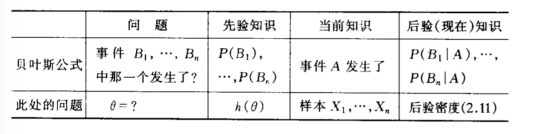
\includegraphics[width=0.8\linewidth]{pic/bayes_estimation}
	
	贝叶斯学派的下一个重要观点:在得出后验分布后,对参数\(\theta\)的任何统计推断,都只能基于这个后验分布。
	
	\textbf{那么如何使用这个后验概率呢?}可以结合某种准则去进行,{\color{red}对点估计问题,一个常用的方法是取后验分布的均值作为\(\theta\)的估计}。
	
	例如,作n次独立试验,每次观察某事件A是否发生,A在每次试验中发生的概率为p,要依据试验结果去估计p
	
	以往都是用频率估计概率的方法去处理。这种方法不用p的先验知识。以下用贝叶斯统计的观点来处理这个问题。
	
	引进\(X_i=1, X_i=0\),视第i次试验时A发生与否而定,\(i=1,...,n. P(X_i=1)=p,P(X_i=0)=1-p\),因此\((X_1,...,X_n)\)的概率函数为\(p^x(1-p)^{n-x}\),x是\(X_i=1\)发生的次数,取p得先验密度h(p),则p的后验密度为
	
	\[h(p|X_1,...,X_n)=\frac{h(p)p^x(1-p)^{n-x}}{\int_{0}^{1}h(p)p^x(1-p)^{n-x}dp}, 0 \leq p \leq 1\]	
	
	此分布的均值(其实就是期望,注意上式得分布是个对p定积分,已经是个无关p的式子了)
	
	\begin{align*}
	\tilde{p}& =\tilde{p}(X_1,...,X_n)=\int_{0}^{1}p h(p|X_1,...,X_n)dp \\
	             & = \frac{\int_{0}^{1}h(p)p^{x+1}(1-p)^{n-x}dp}{\int_{0}^{1}h(p)p^x(1-p)^{n-x}dp}
	\end{align*}
	
	\(\tilde{p}\)就是p在先验分布h(p)之下的贝叶斯估计
	
	上式中概率p是需要进行估计的,h(p)是先验知识,需要我们选择,那么如何选择呢?贝叶斯本人提出过“同等无知”的原则,即实现认为p取[0,1]内一切值都有可能,也就是说在[0,1]内均匀分布,这作为p的先验分布。这时根据均与分布,可知概率密度h(p)=1,当\(0 \leq p \leq 1\),上式的两个积分都可以用\(\beta\)函数表示出,可得:
	
	\[\tilde{p}=\frac{\beta(X+2,n-x+1)}{\beta(X+1,n-x+1)}\]
	
	最终算得
	
	\[\tilde{p}=\frac{X+1}{n+2}\]
	
	这个估计与频率x/n,有些差别,当n很大时并不显著,而在n很小的颇为显著。从一个角度看,当n相当小时,用贝叶斯估计比用x/n合理。因为当n很小的时候,试验结果可能出现X=0或X=n的极端结果,这时,依X/n应该把p估计为0或1,这就太极端了。而在这两种情况下,按照贝叶斯估计,分别给出估计值为1/(n+2)和(n+1)/(n+2)就留有一定的余地。
	
	\textbf{联想:}这跟在自然语言处理里面的平滑处理很像,一句话虽然没有收录在语料库中,或者人们根本不会去说,但不代表这句话不会出现,即出现的概率为0,尤其是某些新词突然出现,比如“蓝瘦香菇”。
	
	\mbox{}
	
	这个同等无知原则也成为贝叶斯原则,被广泛应用到其他情况,不过随着所估计的参数的范围和性质不同,该原则表现的形式也不同。
	
	\mbox{}
	
	\textbf{思考:}其实从贝叶斯的角度来看,极大似然也算是贝叶斯估计的一种,似然函数L其实可以写作\(P(L|\theta)\),本质上也是概率密度函数,只是忽略了先验信息罢了。比如扔硬币,对于似然估计,用频率估计概率,一般都是先做了假设:硬币是均匀材质,正反两面情况出现的机会相等,其实已经利用到了先验信息。但是要是试验的次数很少,只有几次,或者硬币的质地并不均匀,则似然估计就不是那么适用。
	
	贝叶斯公式其实也可以表示成:
	
	\[p(\theta|X)=\frac{p(\theta)p(X|\theta)}{p(X)}=\frac{likelihood·prior}{p(X)}\]
	
	对扔三次硬币,针对不同的先验信息,极大似然以及贝叶斯估计的不同表现
	
	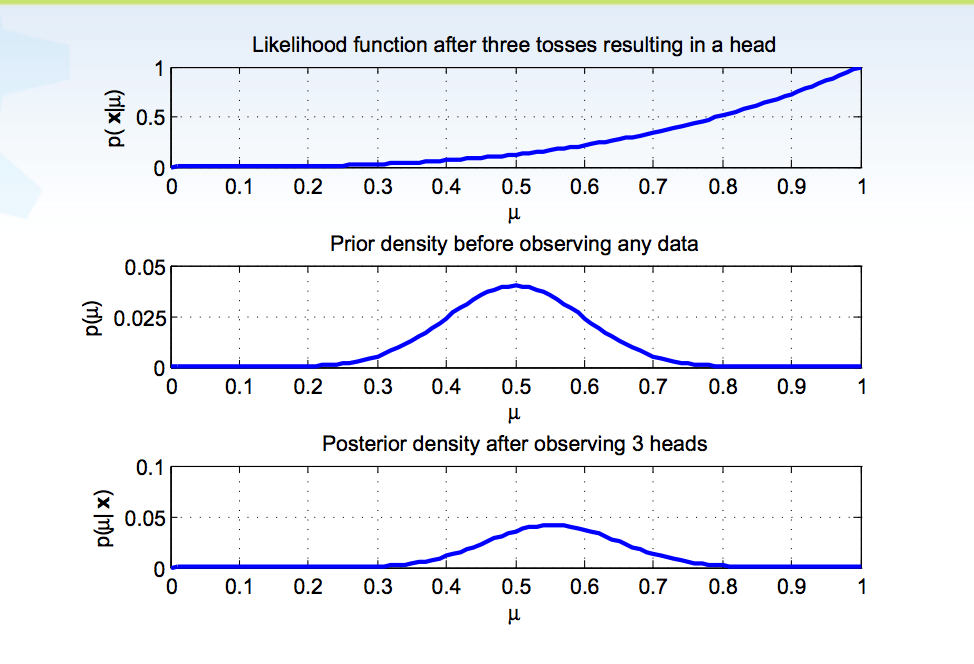
\includegraphics[width=1\linewidth]{pic/prior_and_posterior}
	
	\url{http://www.cs.tut.fi/~hehu/SSP/lecture10.pdf}
	
	
	\subsection{点估计的优良性准则}
	
	在考虑估计量的优劣时,必须从某种整体性能去衡量它,而不能看它在个别样本下得表现如何。整体性有两种意义:一是指估计量的某种特性,具有这种特性就是好的,否则就是不好的,如无偏性;二是指某种具体的数量性指标,两个估计量,指标小者为优,比如均方误差。
	
	\mbox{}
	
	\textbf{估计量的无偏性}
	
	设某统计总体的分布包含未知参数\(\theta_1,...,\theta_k, X_1,...,X_n\)是从该总体抽出的样本,要估计\(g(\theta_1,...,\theta_k)\)。g为一已知函数。设\(\hat{g}(X_1,...,X_n)\)是一个估计量,如果对任何可能的\(\theta_1,...,\theta_k\)都有
	
	\[E_{\theta_1,...,\theta_k}[\hat{g}(X_1,...,X_n)] = g(\theta_1,...,\theta_k)\]
	
	称\(\hat{g}\)是\(g(\theta_1,...,\theta_k)\)的一个无偏估计量。
	
	估计量的无偏性有两个含义。第一个含义是没有系统性的偏差,不论用什么样的估计量\(\hat{g}\)去估计g,总是时而偏低,时而偏高。无偏性表示,把这些正负偏差在概率上平均起来,其值为0.
	
	另一个含义是估计量由无偏性,则在大量次数使用取平均时,能以接近于100\%的把握无限逼近被估计量。如果没有无偏性,则无论是用多少次,其平均也会与真值保持一定距离——这距离就是系统误差
	
	\mbox{}
	
	\textbf{最小方差无偏估计}
	
	一个参数往往有不止一个无偏估计,从这些众多的无偏估计中,挑选出最优的。这牵涉到两个问题:一是为优良性制定一个准则,二是在已定的准则之下,如何找到最优者。
	
	1.均方误差,设\(X_1,...,X_n\)是从某一带参数\(\theta\)的总体中抽出的样本,要估计\(\theta\).若我们采用估计量\(\hat{\theta}=\hat{\theta}(X_1,...,X_n)\),则其误差为\(\hat{\theta}(X_1,...,X_n)-\theta\).这误差随样本\(X_1,...,X_n\)的具体值而定,也是随机的,因为其本身无法取为优良性指标。我们把它平方以消除符号,得\((\hat{\theta}(X_1,..,X_n)-\theta)^2\),然后取它的均值:
	
	\[M_{\hat{\theta}}(\theta)=E_{\theta}[\hat{\theta}(X_1,...,X_n)-\theta]^2\]
	
	2.最小方差无偏估计(MVU估计)。若局限于无偏估计的范围,且采用均方误差的准则,则两个无偏估计\(\hat{\theta}_1\)和\(\hat{\theta}_2\)的比较,归结为其方差的比较:方差小者为优
	
	\mbox{}
	
	\textbf{估计量的相合性与渐近正态性}
	
	\textbf{定义:}设总体分布依赖于参数\(\theta_1,...,\theta_k\), \(g(\theta_1,...,\theta_k)\)是\(\theta_1,...,\theta_k\)之一给定函数。设\(X_1,X_2,...,X_n\)为该总体中抽出的样本,\(T(X_1,...,X_n)\)是\(g(\theta_1,...,\theta_k)\)的一个估计量,如果对任意给定的\(\varepsilon > 0\)有
	
	\[\lim\limits_{n \to \infty}P_{\theta_1,..,\theta_k}(|T(X_1,...,X_n)-g(\theta_1,...,\theta_k)| \geq \varepsilon) = 0\]
	
	而且这对\(\theta_1,...,\theta_k\)一切可能取的值都成立,则称\(T(X_1,...,X_n)\)是\(g(\theta_1,...,\theta_k)\)的一个相合估计。
	
	如果当样本大小无限增加时,估计量依概率收敛于被估计的值,则称该估计量是相合估计。
	
	渐近正态性:当样本大小\(n \to \infty\)时,其分布都渐近于正态分布
	
	\textbf{总结:}估计量的相合性和渐近正态性成为估计量的大样本性质,指的是:这种性质都是对样本大小\(n \to \infty\)来谈的,对一个固定的n,相合性与渐近正态性都是无意义。与此相对,估计量的无偏性概念是对固定的样本大小来谈的,不需要样本大小趋于无穷。这种性质成为小样本性质。因此大小样本性质之分不在于样本的具体大小如何,而在于样本大小趋于无穷与否。
	
	\subsection{区间估计}
	
	设\(X_1,...,X_n\)是从该总体中抽出的样本。所谓\(\theta\)的区间估计,就是满足条件\(\hat{\theta}_1(X_1,...,X_n) < \hat{\theta}_2(X_1,...,X_n)\)的两个统计量\(\hat{\theta_1},\hat{\theta_2}\)为端点的区间\([\hat{\theta_1},\hat{\theta_2}]\)。一旦有了样本\(X_1,...,X_n\),就把\(\theta\)估计在区间\([\hat{\theta}_1(X_1,...,X_n) , \hat{\theta}_2(X_1,...,X_n)]\)之内,这里有两个要求:
	
	1.\(\theta\)要以很大的可能性落在区间\([\hat{\theta_1},\hat{\theta_2}]\)内,也就是说,概率\(P_\theta(\hat{\theta}_1(X_1,...,X_n) \leq \theta \leq \hat{\theta}_2(X_1,...,X_n))\)要尽可能大
	
	2.估计的精密度要尽可能高。区间的长度尽可能小
	
	\textbf{定义:}给定一个很小的数\(\alpha > 0\)。如果对参数\(\theta\)的任何值,概率\(P_\theta(\hat{\theta}_1(X_1,...,X_n) \leq \theta \leq \hat{\theta}_2(X_1,...,X_n))\)都等于\(1-\alpha\),则称区间估计\([\hat{\theta_1},\hat{\theta_2}]\)的置信系数为\(1-\alpha\).
	
	区间估计也常称为置信区间。意思是对该区间能包含未知参数\(\theta\)可置信到何种程度。
	
	构造合理的区间估计的方法:
	
	\textbf{枢轴变量法}
	
	例如,设\(X_1,...,X_n\)为抽自正态总体\(N(\mu, \sigma^2)\)的样本,{\color{red}\(\sigma^2\)}已知,要求\(\mu\)的区间估计
	
	{\color{red}先找一个\(\mu\)的良好的点估计},在此可以选择样本均值\(\overline{X}\)。由总体为正态易知
	
	\[\sqrt{n}(\overline{X}-\mu)/\sigma \sim N(0, 1)\]
	
	以\(\varPhi\)记为N(0,1)的分布函数。对\(0 < \beta < 1\),用方程
	
	\[\varPhi(\mu_\beta)=1-\beta\]
	
	定义记号\(\mu_\beta\)为分布N(0,1)的上\(\beta\)分位点。其意义是:N(0,1)分布中大于\(\mu_\beta\)的那部分的概率就是\(\beta\).如下图画的是N(0,1)的密度函数,涂黑的部分标出的面积就是\(\beta\)
	
	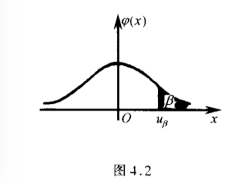
\includegraphics[width=0.8\linewidth]{pic/beta}
	
	由上面的式子以及\(\varPhi(-t)=1-\varPhi(t)\)有
	
	\begin{align*}
	P(-\mu_{\alpha/2} \leq \sqrt{n}(\overline{X}-\mu)/\sigma \leq \mu_{\alpha/2} & = \varPhi(\mu_{\alpha/2})-\varPhi(\mu_{\alpha/2}) \\
			& = (1-\alpha/2)-\alpha/2 = 1- \alpha
	\end{align*}
	
	可以改写为:
	
	\[P(\overline{X}-\sigma\mu_{\alpha/2}/\sqrt{n} \leq \mu \leq \overline{X}+\sigma\mu_{\alpha/2}/\sqrt{n})\]
	
	此式指出:
	
	\[[\hat{\theta_1},\hat{\theta_2}]=[\overline{X}-\sigma\mu_{\alpha/2}/\sqrt{n}, \overline{X}+\sigma\mu_{\alpha/2}/\sqrt{n}]\]
	
	可作为\(\mu\)的区间估计,置信系数为\(1-\alpha\)
	
	方法可总结为:
	
	1.找到一个与要估计的参数\(g(\theta)\)有关的统计量T,一般是其良好的点估计(此例T为\(\overline{X}\)
	
	2.设法找出T和\(g(\theta)\)的某一函数\(S(T,g(\theta))\),其分布F要与\(\theta\)无关(此例中,\(S(T,g(\theta))\)为\(\sqrt{n}(\overline{X}-\mu)/\sigma\),分布F就是\(\varPhi\).S成为枢轴变量。
	
	3.对任何常数a < b,不等式\(a \leq S(T,g(\theta)) \leq b\)要能够改写成为等价的形式\(A \leq g(\theta) \leq B\),A,B只与T,a,b有关而与\(\theta\)无关
	
	4.取分布F的上\(\alpha/2\)分位点\(\omega_{\aleph/2}\)和上\(1-\alpha/2\)分位点\(\omega_{1-\aleph/2}\)。有\(F(\omega_{\aleph/2})-F(\omega_{1-\aleph/2})=1-\alpha\),因此
	
	\[P(\omega_{1-\aleph/2} \leq S(T, g(\theta)) \leq \omega_{\aleph/2})=1-\alpha\]
	
	得到某个具体的区间后,\(\mu\)是一个虽然未知,但其值确定的数。区间包含\(\mu\),或者不包含,二者只居其一。说这区间的置信系数是0.95,其确切的意义应当是:它是根据所有的数据,用一个置信系数为0.95的方法作出的。可见置信系数一词是针对方法:用这方法作出的区间估计,平均100此种95次包含所要估计的值。一旦算出具体区间,就不能再说它有95\%的机会包含要估计的值了。比如一个人擅长挑选西瓜:他挑选的西瓜,平均100个中有95个好的。某天他给你挑一个,结果或好或坏,必居其一,不是95\%的好。但是考虑到它挑瓜的技术,我对他挑的比较放心,这就是置信系数。
	
	\textbf{大样本法}
	
	主要利用中心极限定理,以建立枢轴变量
	
	\textbf{贝叶斯法}
	
	在有了先验分布密度\(h(\theta)\)和样本\(X_1,...,X_n\)后,算出后验密度\(h(\theta|X_1,..,X_n)\),再找两个数\(\hat{\theta_1}, \hat{\theta_2}\)都与\(X_1,...,X_n\)有关,使得:
	
	\[\int_{\hat{\theta_1}}^{\hat{\theta_2}}h(\theta|X_1,...,X_n)d\theta = 1-\alpha\]
	
	区间\(\hat{\theta_1}, \hat{\theta_2}\)的意思是:在所得后验分布之下,\(\theta\)落在这区间的概率为\(1-\alpha\)
	
	\section{假设检验}
	
	
	
	
	
	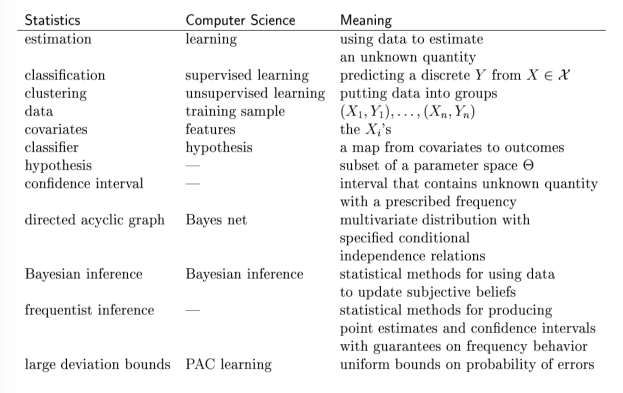
\includegraphics[width=0.8\linewidth]{pic/statistics_data_mining_dict}
	
	\section{不等式}
	
	\subsection{Markov and Chebychev Inequalities}
	
	\textbf{Markov's Inequality:}
	X是非负的随机变量,同时假设E(X)存在,对任意的t>0,有:
	
	\[P(X> t) \leq \frac{E(X)}{t}\]
	
	\textbf{PROOF:}
	
	\begin{align*}
	E(X)=\int_{0}^{\infty}xf(x)dx& =\int_{0}^{t}xf(x)dx+\int_{t}^{\infty}xf(x)dx \\
	 & \geq \int_{t}^{\infty}xf(x)dx \\
	 & \geq t\int_{t}^{\infty}f(x)dx = tP(X>t)
	\end{align*}
	
	\textbf{Chebyshev's inequality:}
	让\(\mu=E(X), \sigma^2=V(X)\),然后有:
	
	\[P(|X-\mu| \geq t) \leq \frac{\sigma^2}{t^2} , P(|Z| \geq k) \leq \frac{1}{k^2}, Z=(X-\mu)/\sigma\]
	
	\textbf{PROOF:}
	
	use Markov's inequality to conclude that:
	
	\[P(|X-\mu| \geq t) = P(|X-\mu|^2 \geq t^2) \leq \frac{E(X-\mu)^2}{t^2}=\frac{\sigma^2}{t^2}\]
	
	the second part follows by setting \(t = k\sigma\)
	
	\[P(|X-\mu|) \geq k\sigma) = P(|X-\mu|/\sigma \geq k) = P(|Z| \geq k) \leq \frac{1}{k^2}\]

	\subsection{Hoeffding's Inequality}
	
	\textbf{Theorem:}
	
	let \(Y_1,...,Y_n\) be independent observations such that \(E(Y_i) = 0\),and \(a_i \leq Y_i \leq b_i, \epsilon > 0\), for any t > 0
	
	\[P(\sum_{i=1}^{n}Y_i \geq \epsilon) \leq e^{-t\epsilon}\prod_{i=1}^{n}e^{t^2(b_i-a_i)^2/8}\]
	
	\textbf{Theorem:}
	
	let \(X_1,...,X_n \sim Bernoulli(p)\), then for any \(\epsilon > 0\),
	
	\[P(|\overline{X}_n-p| > \epsilon) \leq 2e^{-2n\epsilon^2}, \overline{X}_n=\sum_{i=1}^{n}X_i/n\]
	
	Fix \(\alpha > 0\) and let
	
	\[\epsilon_n = \{\frac{1}{2n}\log(\frac{2}{\alpha})\}^{1/2}\]
	
	By Hoeffding's inequality,
	
	\[P(|\overline{X}_n-p| > \epsilon) \leq 2e^{-2n\epsilon^2} = \alpha\]
	
	let \(C = (\overline{X}_n-\epsilon, \overline{X}_n+\epsilon)\).
	
	\[P(p \notin C) = P(|\overline{X}_n-p| > \epsilon) \leq \alpha\]
	
	So
	
	\[P(p \in C) \geq 1-\alpha\]
	
	所以随机变量p以\(1-\alpha\)的概率落在随机区间C中
	
	\subsection{Cauchy-Schwarz and Jensen Inequalities}
	
	\textbf{Cauchy-Schwarz inequality:} If X and Y have inite variances then
	
	\[E|XY| \leq \sqrt{E(X^2)E(Y^2)}\]
	
	\textbf{Jensen's Inequality:} If g is convex then
	
	\[Eg(X) \geq g(EX)\]
	
	if g is concave then
	
	\[Eg(X) \leq g(EX)\]
	
	\textbf{PROOF:}
	
	假设直线L(x)=a+bx,与g(x)的切点在E(X),因为g是凸函数,曲线位于直线L之上,所以
	
	\[Eg(X) \geq E(L)=E(a+bX)=a+bE(X)=L(E(X))=g(E(X))\]
	
	由上式可知,\(EX^2 \geq (EX)^2, E(1/X) \geq 1/E(X)\)
	
	
	
	
	
	
	\begin{thebibliography}{99}
		\bibitem{ref1}陈希孺:概率论与数理统计
		\bibitem{ref2}茆诗松:贝叶斯统计
		\bibitem{ref3}all of statistics
	\end{thebibliography}
\end{document}